
%% bare_conf.tex
%% V1.4b
%% 2015/08/26
%% by Michael Shell
%% See:
%% http://www.michaelshell.org/
%% for current contact information.
%%
%% This is a skeleton file demonstrating the use of IEEEtran.cls
%% (requires IEEEtran.cls version 1.8b or later) with an IEEE
%% conference paper.
%%
%% Support sites:
%% http://www.michaelshell.org/tex/ieeetran/
%% http://www.ctan.org/pkg/ieeetran
%% and
%% http://www.ieee.org/

%%*************************************************************************
%% Legal Notice:
%% This code is offered as-is without any warranty either expressed or
%% implied; without even the implied warranty of MERCHANTABILITY or
%% FITNESS FOR A PARTICULAR PURPOSE! 
%% User assumes all risk.
%% In no event shall the IEEE or any contributor to this code be liable for
%% any damages or losses, including, but not limited to, incidental,
%% consequential, or any other damages, resulting from the use or misuse
%% of any information contained here.
%%
%% All comments are the opinions of their respective authors and are not
%% necessarily endorsed by the IEEE.
%%
%% This work is distributed under the LaTeX Project Public License (LPPL)
%% ( http://www.latex-project.org/ ) version 1.3, and may be freely used,
%% distributed and modified. A copy of the LPPL, version 1.3, is included
%% in the base LaTeX documentation of all distributions of LaTeX released
%% 2003/12/01 or later.
%% Retain all contribution notices and credits.
%% ** Modified files should be clearly indicated as such, including  **
%% ** renaming them and changing author support contact information. **
%%*************************************************************************


% *** Authors should verify (and, if needed, correct) their LaTeX system  ***
% *** with the testflow diagnostic prior to trusting their LaTeX platform ***
% *** with production work. The IEEE's font choices and paper sizes can   ***
% *** trigger bugs that do not appear when using other class files.       ***                          ***
% The testflow support page is at:
% http://www.michaelshell.org/tex/testflow/



\documentclass[conference]{IEEEtran}
% Some Computer Society conferences also require the compsoc mode option,
% but others use the standard conference format.
%
% If IEEEtran.cls has not been installed into the LaTeX system files,
% manually specify the path to it like:
% \documentclass[conference]{../sty/IEEEtran}





% Some very useful LaTeX packages include:
% (uncomment the ones you want to load)


% *** MISC UTILITY PACKAGES ***
%
\usepackage{ifpdf}
% Heiko Oberdiek's ifpdf.sty is very useful if you need conditional
% compilation based on whether the output is pdf or dvi.
% usage:
% \ifpdf
%   % pdf code
% \else
%   % dvi code
% \fi
% The latest version of ifpdf.sty can be obtained from:
% http://www.ctan.org/pkg/ifpdf
% Also, note that IEEEtran.cls V1.7 and later provides a builtin
% \ifCLASSINFOpdf conditional that works the same way.
% When switching from latex to pdflatex and vice-versa, the compiler may
% have to be run twice to clear warning/error messages.






% *** CITATION PACKAGES ***
%
\usepackage{cite}
% cite.sty was written by Donald Arseneau
% V1.6 and later of IEEEtran pre-defines the format of the cite.sty package
% \cite{} output to follow that of the IEEE. Loading the cite package will
% result in citation numbers being automatically sorted and properly
% "compressed/ranged". e.g., [1], [9], [2], [7], [5], [6] without using
% cite.sty will become [1], [2], [5]--[7], [9] using cite.sty. cite.sty's
% \cite will automatically add leading space, if needed. Use cite.sty's
% noadjust option (cite.sty V3.8 and later) if you want to turn this off
% such as if a citation ever needs to be enclosed in parenthesis.
% cite.sty is already installed on most LaTeX systems. Be sure and use
% version 5.0 (2009-03-20) and later if using hyperref.sty.
% The latest version can be obtained at:
% http://www.ctan.org/pkg/cite
% The documentation is contained in the cite.sty file itself.



% *** GRAPHICS RELATED PACKAGES ***
%
%\ifCLASSINFOpdf
%  % \usepackage[pdftex]{graphicx}
%  % declare the path(s) where your graphic files are
%  % \graphicspath{{../pdf/}{../jpeg/}}
%  % and their extensions so you won't have to specify these with
%  % every instance of \includegraphics
%  % \DeclareGraphicsExtensions{.pdf,.jpeg,.png}
%\else
%  % or other class option (dvipsone, dvipdf, if not using dvips). graphicx
%  % will default to the driver specified in the system graphics.cfg if no
%  % driver is specified.
%  % \usepackage[dvips]{graphicx}
%  % declare the path(s) where your graphic files are
%  % \graphicspath{{../eps/}}
%  % and their extensions so you won't have to specify these with
%  % every instance of \includegraphics
%  % \DeclareGraphicsExtensions{.eps}
%\fi
% graphicx was written by David Carlisle and Sebastian Rahtz. It is
% required if you want graphics, photos, etc. graphicx.sty is already
% installed on most LaTeX systems. The latest version and documentation
% can be obtained at: 
% http://www.ctan.org/pkg/graphicx
% Another good source of documentation is "Using Imported Graphics in
% LaTeX2e" by Keith Reckdahl which can be found at:
% http://www.ctan.org/pkg/epslatex
%
% latex, and pdflatex in dvi mode, support graphics in encapsulated
% postscript (.eps) format. pdflatex in pdf mode supports graphics
% in .pdf, .jpeg, .png and .mps (metapost) formats. Users should ensure
% that all non-photo figures use a vector format (.eps, .pdf, .mps) and
% not a bitmapped formats (.jpeg, .png). The IEEE frowns on bitmapped formats
% which can result in "jaggedy"/blurry rendering of lines and letters as
% well as large increases in file sizes.
%
% You can find documentation about the pdfTeX application at:
% http://www.tug.org/applications/pdftex





% *** MATH PACKAGES ***
%
\usepackage{amsmath}
% A popular package from the American Mathematical Society that provides
% many useful and powerful commands for dealing with mathematics.
%
% Note that the amsmath package sets \interdisplaylinepenalty to 10000
% thus preventing page breaks from occurring within multiline equations. Use:
%\interdisplaylinepenalty=2500
% after loading amsmath to restore such page breaks as IEEEtran.cls normally
% does. amsmath.sty is already installed on most LaTeX systems. The latest
% version and documentation can be obtained at:
% http://www.ctan.org/pkg/amsmath





% *** SPECIALIZED LIST PACKAGES ***
%
%\usepackage{algorithmic}
% algorithmic.sty was written by Peter Williams and Rogerio Brito.
% This package provides an algorithmic environment fo describing algorithms.
% You can use the algorithmic environment in-text or within a figure
% environment to provide for a floating algorithm. Do NOT use the algorithm
% floating environment provided by algorithm.sty (by the same authors) or
% algorithm2e.sty (by Christophe Fiorio) as the IEEE does not use dedicated
% algorithm float types and packages that provide these will not provide
% correct IEEE style captions. The latest version and documentation of
% algorithmic.sty can be obtained at:
% http://www.ctan.org/pkg/algorithms
% Also of interest may be the (relatively newer and more customizable)
% algorithmicx.sty package by Szasz Janos:
% http://www.ctan.org/pkg/algorithmicx




% *** ALIGNMENT PACKAGES ***
%
%\usepackage{array}
% Frank Mittelbach's and David Carlisle's array.sty patches and improves
% the standard LaTeX2e array and tabular environments to provide better
% appearance and additional user controls. As the default LaTeX2e table
% generation code is lacking to the point of almost being broken with
% respect to the quality of the end results, all users are strongly
% advised to use an enhanced (at the very least that provided by array.sty)
% set of table tools. array.sty is already installed on most systems. The
% latest version and documentation can be obtained at:
% http://www.ctan.org/pkg/array


% IEEEtran contains the IEEEeqnarray family of commands that can be used to
% generate multiline equations as well as matrices, tables, etc., of high
% quality.




% *** SUBFIGURE PACKAGES ***
%\ifCLASSOPTIONcompsoc
%  \usepackage[caption=false,font=normalsize,labelfont=sf,textfont=sf]{subfig}
%\else
%  \usepackage[caption=false,font=footnotesize]{subfig}
%\fi
% subfig.sty, written by Steven Douglas Cochran, is the modern replacement
% for subfigure.sty, the latter of which is no longer maintained and is
% incompatible with some LaTeX packages including fixltx2e. However,
% subfig.sty requires and automatically loads Axel Sommerfeldt's caption.sty
% which will override IEEEtran.cls' handling of captions and this will result
% in non-IEEE style figure/table captions. To prevent this problem, be sure
% and invoke subfig.sty's "caption=false" package option (available since
% subfig.sty version 1.3, 2005/06/28) as this is will preserve IEEEtran.cls
% handling of captions.
% Note that the Computer Society format requires a larger sans serif font
% than the serif footnote size font used in traditional IEEE formatting
% and thus the need to invoke different subfig.sty package options depending
% on whether compsoc mode has been enabled.
%
% The latest version and documentation of subfig.sty can be obtained at:
% http://www.ctan.org/pkg/subfig




% *** FLOAT PACKAGES ***
%
%\usepackage{fixltx2e}
% fixltx2e, the successor to the earlier fix2col.sty, was written by
% Frank Mittelbach and David Carlisle. This package corrects a few problems
% in the LaTeX2e kernel, the most notable of which is that in current
% LaTeX2e releases, the ordering of single and double column floats is not
% guaranteed to be preserved. Thus, an unpatched LaTeX2e can allow a
% single column figure to be placed prior to an earlier double column
% figure.
% Be aware that LaTeX2e kernels dated 2015 and later have fixltx2e.sty's
% corrections already built into the system in which case a warning will
% be issued if an attempt is made to load fixltx2e.sty as it is no longer
% needed.
% The latest version and documentation can be found at:
% http://www.ctan.org/pkg/fixltx2e


\usepackage{stfloats}
% stfloats.sty was written by Sigitas Tolusis. This package gives LaTeX2e
% the ability to do double column floats at the bottom of the page as well
% as the top. (e.g., "\begin{figure*}[!b]" is not normally possible in
% LaTeX2e). It also provides a command:
%\fnbelowfloat
% to enable the placement of footnotes below bottom floats (the standard
% LaTeX2e kernel puts them above bottom floats). This is an invasive package
% which rewrites many portions of the LaTeX2e float routines. It may not work
% with other packages that modify the LaTeX2e float routines. The latest
% version and documentation can be obtained at:
% http://www.ctan.org/pkg/stfloats
% Do not use the stfloats baselinefloat ability as the IEEE does not allow
% \baselineskip to stretch. Authors submitting work to the IEEE should note
% that the IEEE rarely uses double column equations and that authors should try
% to avoid such use. Do not be tempted to use the cuted.sty or midfloat.sty
% packages (also by Sigitas Tolusis) as the IEEE does not format its papers in
% such ways.
% Do not attempt to use stfloats with fixltx2e as they are incompatible.
% Instead, use Morten Hogholm'a dblfloatfix which combines the features
% of both fixltx2e and stfloats:
%
% \usepackage{dblfloatfix}
% The latest version can be found at:
% http://www.ctan.org/pkg/dblfloatfix




% *** PDF, URL AND HYPERLINK PACKAGES ***
%
\usepackage{url}
% url.sty was written by Donald Arseneau. It provides better support for
% handling and breaking URLs. url.sty is already installed on most LaTeX
% systems. The latest version and documentation can be obtained at:
% http://www.ctan.org/pkg/url
% Basically, \url{my_url_here}.




% *** Do not adjust lengths that control margins, column widths, etc. ***
% *** Do not use packages that alter fonts (such as pslatex).         ***
% There should be no need to do such things with IEEEtran.cls V1.6 and later.
% (Unless specifically asked to do so by the journal or conference you plan
% to submit to, of course. )


% correct bad hyphenation here
\hyphenation{op-tical net-works semi-conduc-tor}


\begin{document}
%
% paper title
% Titles are generally capitalized except for words such as a, an, and, as,
% at, but, by, for, in, nor, of, on, or, the, to and up, which are usually
% not capitalized unless they are the first or last word of the title.
% Linebreaks \\ can be used within to get better formatting as desired.
% Do not put math or special symbols in the title.
\title{Human Robot Interaction\\ in an Airport}


% author names and affiliations
% use a multiple column layout for up to three different
% affiliations
%\author{\IEEEauthorblockN{Michael Shell}
%\IEEEauthorblockA{School of Electrical and\\Computer Engineering\\
%Georgia Institute of Technology\\
%Atlanta, Georgia 30332--0250\\
%Email: http://www.michaelshell.org/contact.html}
%\and
%\IEEEauthorblockN{Homer Simpson}
%\IEEEauthorblockA{Twentieth Century Fox\\
%Springfield, USA\\
%Email: homer@thesimpsons.com}
%\and
%\IEEEauthorblockN{James Kirk\\ and Montgomery Scott}
%\IEEEauthorblockA{Starfleet Academy\\
%San Francisco, California 96678--2391\\
%Telephone: (800) 555--1212\\
%Fax: (888) 555--1212}}

% conference papers do not typically use \thanks and this command
% is locked out in conference mode. If really needed, such as for
% the acknowledgment of grants, issue a \IEEEoverridecommandlockouts
% after \documentclass

% for over three affiliations, or if they all won't fit within the width
% of the page, use this alternative format:
% 
\author{\IEEEauthorblockN{Andreas Kornmaaler Hansen\IEEEauthorrefmark{0},
Emil Bonnerup\IEEEauthorrefmark{0},
Juliane Nilsson\IEEEauthorrefmark{0}, 
Lucca Julie Nellemann,\IEEEauthorrefmark{0} and
Sara Nielsen\IEEEauthorrefmark{0}}
\IEEEauthorblockA{\IEEEauthorrefmark{0}School of Information and Communication Technology\\
Aalborg University,
Aalborg, Denmark\\ Email: 17gr782@es.aau.dk}
}


\makeatletter
\def\bstctlcite{\@ifnextchar[{\@bstctlcite}{\@bstctlcite[@auxout]}}
\def\@bstctlcite[#1]#2{\@bsphack
  \@for\@citeb:=#2\do{%
    \edef\@citeb{\expandafter\@firstofone\@citeb}%
    \if@filesw\immediate\write\csname #1\endcsname{\string\citation{\@citeb}}\fi}%
  \@esphack}
\makeatother

% use for special paper notices
%\IEEEspecialpapernotice{(Invited Paper)}




% make the title area
\maketitle

% As a general rule, do not put math, special symbols or citations
% in the abstract
\begin{abstract}
\label{Abstract}
% As a general rule, do not put math, special symbols or citations
% in the abstract
Social robots are expected to play a much bigger role in the near future. This calls for research in determining how these social robots are supposed to behave. This paper presents an ecological field study and investigates the subjective experience of social robots in Aalborg Airport (AAL). Travellers were recruited by a remote controlled robot from Double Robotics, Inc., which had a tablet with an interface asking if it may help them with wayfinding in AAL. When the participants had chosen their location they were asked to follow the robot and led to a semi-structured interview about their first impressions. In total the study includes 30 participants from 8 to 62 years (M=37.9, SD=17.1). The observations and the participants' statements were coded using an Affinity Diagram. 567 affinity notes were sorted and ended up with 10 categories of which the main categories revolved around appearance, behaviour, approach and trust. 


%method
%result
%conclusion

\end{abstract}

% no keywords




% For peer review papers, you can put extra information on the cover
% page as needed:
% \ifCLASSOPTIONpeerreview
% \begin{center} \bfseries EDICS Category: 3-BBND \end{center}
% \fi
%
% For peerreview papers, this IEEEtran command inserts a page break and
% creates the second title. It will be ignored for other modes.
\IEEEpeerreviewmaketitle



\chapter*{Introduction}
\label{introduction}
%
The goal of this paper is to analyse results from a study called \textit{Men and Bread} using Principal Component Analysis (PCA). \blankline
% 
<<<<<<< HEAD
In the study \textit{Men and Bread}, 21 subjects were asked to rate different types of buns according to different attributes. Nine different types of buns were presented, where one was presented as a familiarization with the scales. The buns presented in the study are shown in \autoref{fig:bread}, where bread B9 is the bun used for familiarization. 
=======
In the study \textit{Men and Bread} 21 subjects were asked to rate nine different types of buns according to different attributes. Nine different types of buns were presented where one was presented as a familiarization with the scales. The buns presented in the study are shown on \autoref{fig:bread}, where bread B9 is the bun used for familiarization. 
>>>>>>> ad024fa761c2fdb0b59931c6f6a1eb4b88ee637a
%
\begin{figure}[H]
\centering
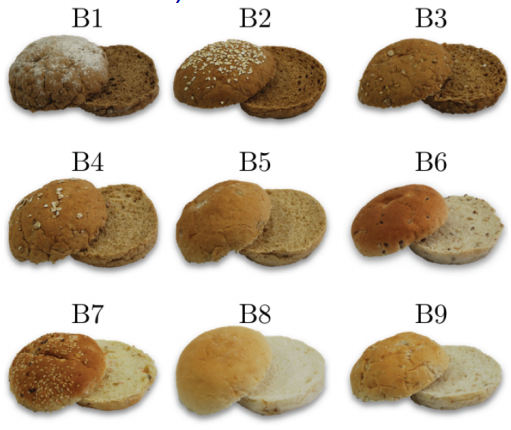
\includegraphics[width =0.7\textwidth]{Figure/Bread}
\caption{The different types of buns with identifying name, presented so that both crust and crumb can be seen.}
\label{fig:bread}
\end{figure}
\noindent
%
For each one of the different types of buns, 11 different attributes grouped in three different categories were rated. The attributes with the belonging scale question for each category are presented in \autoref{tab:DirectPerception}, \autoref{tab:AbstractPerception}, and \autoref{tab:Reflection}.
%
\begin{table}[H]
	\centering 
	\begin{tabular}{ |l|l| }
	\hline
	\multicolumn{2}{ |c| }{\textbf{Direct perception}} \\
	\hline
	\textit{Attribute} & \textit{Scale Question} \\ 
	\hline
	\multirow{2}{*}{Crust} & Hvilken farve har skorpen? (lys til mørk) \\
 	&  What color is the crust? (light to dark) \\ \hline
	\multirow{2}{*}{Crumb} &  Hvilken farve har krummen? (lys til mørk) \\
 	&  What color is the crumb? (light to dark) \\ \hline
	\multirow{2}{*}{Surface} & Hvilken tekstur har overfladen? (glat til ujævn) \\
 	&  What texture does the surface have? (smooth to uneven) \\ \hline
	\multirow{2}{*}{Seeds} & Hvor stor er andelen af kerner? (lav til høj) \\ 
 	&  How great is the amount of seeds? (small to large)\\ 
	\hline
	\end{tabular}
	\caption{Scale questions under the category: Direct perception. This category of questions are related to the readily available aspects of the bread.}
	\label{tab:DirectPerception}       
\end{table}
\noindent
%
\begin{table}[H]
	\centering 
	\begin{tabular}{ |l|l| }
	\hline
	\multicolumn{2}{ |c| }{\textbf{Abstract perception}} \\
	\hline
	\textit{Attribute} & \textit{Scale Question} \\ 
	\hline
	\multirow{2}{*}{Weight} &  Hvor tungt er brødet? (let til tungt) \\
 	&  How weighty is the bread? (light to heavy) \\ \hline
	\multirow{2}{*}{Density} & Hvor tæt er brødet? (luftigt til kompakt) \\
 	&  How dense is the bread? (airy to dense) \\ \hline
	\multirow{2}{*}{Juicy} &  Hvor saftigt er brødet? (tørt til svampet) \\
 	&  How juicy is the bread? (dry to moist) \\ 
 	\hline
	\end{tabular}
	\caption{Scale questions under the category: Abstract perception. This category relates to slightly more abstract concepts where the visual sense might not be the best tool for investigation.}
	\label{tab:AbstractPerception}       
\end{table}
\noindent
%
\begin{table}[H]
	\centering 
	\begin{tabular}{ |l|l| }
	\hline
	\multicolumn{2}{ |c| }{\textbf{Reflection}} \\
	\hline
	\textit{Attribute} & \textit{Scale Question} \\ 
	\hline
	\multirow{2}{*}{Filling} & Hvor mættende ser brødet ud? (lidt til meget) \\
 	&  How filling is the bread? (a little to a lot) \\ \hline
	\multirow{2}{*}{Nourishing} & Hvor nærende ser brødet ud? (usundt til sundt) \\
 	&   How nourishing is the bread? (healthy to unhealthy) \\ \hline
	\multirow{2}{*}{Wholegrain} & Hvor fuldkornsholdigt er brødet? (lidt til meget) \\
 	&   How large is the amount of wholegrain in the bread? (low to high) \\ \hline
	\multirow{2}{*}{Fibre} & Hvor fiberholdigt er brødet? (lidt til meget) \\ 
 	&   How fibrous is the bread? (low to high))\\ 
	\hline
	\end{tabular}
	\caption{Scale questions under the category: Reflection. This category concerns the qualities associated with bread. Qualities which are assumed to require a level of reflection.}
	\label{tab:Reflection}       
\end{table}
\noindent
%
Each scale question were presented to the test subjects with a scale. The scale used to rate the buns was a \textit{Visual Analogue Scale} (VAS) with open endpoints and an anchor point in the middle. An example of the scale used in the study is shown on \autoref{fig:Skala}. 
%
\begin{figure}[H]
\centering
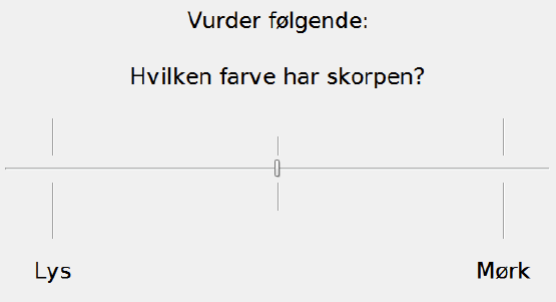
\includegraphics[width =0.7\textwidth]{Figure/Skala}
\caption{Example of the VAS used in the study \textit{Men and Bread}.}
\label{fig:Skala}
\end{figure}
\noindent


%Analyze the results from the example using PCA.

%First plot a “profile” of all stimuli.

%How much of the variance is explained by each component?

%(Plot a scree-plot including cumulative variance).

%Plot your PCA solution graphically. Both a plot with just your stimuli (scores) and a biplot with both scores and loadings.

%Make a table of the loadings of each word-pair on each principal component.

%Interpret the solution. Also, are there word-pairs that seem ”redundant” e.g. measures that same perceptual attribute?


\section*{Method}
\label{Method}
%
In order to know whether or not the BTL model can be applied to the data shown in \autoref{tab:data}, it is first necessary to check for transitivity in the data. In other words how reliable and consistent the data is. The cumulative preference matrix is a pooled data matrix meaning it contains data from all the participants deemed sufficiently consistent. This is typically done using a $\chi^{2}-test$. Now a problem could arise because it is unknown whether the pooled subjects have shown an opposite decision behaviour eg. chosen pleasant where others chose unpleasant or not. If that is the case, then the preference matrix becomes inconsistent. Before it is possible to do the transitivity check, it is necessary to calculate the probability of a stimulus being rated as unpleasant. See \autoref{eg:probability}.
%
\begin{equation}
p = \frac{freq}{n}
\end{equation}
\noindent
%
Here \textit{freq} is the frequency that a sound has been rated unpleasant (the pooled preference matrix, \autoref{tab:data}) and \textit{n} is the number of test subjects. Thereafter it is needed to check every combination of the stimuli for transitivity violations. There are no set rules but a rough estimate of when the probabilistic choice models holds is shown in \autoref{tab:trans_violations}:
%
\begin{table}[H]
\centering
\begin{tabular}{@{}ll@{}}
\toprule
Transitivity violations                                    & Expected                                      \\ \midrule
None or few SST violations                                 & BTL may fit                                   \\
Some SST violations and few MST violations                 & Preference-tree might fit (Not BTL)            \\
Considerable SST and MST but few WST violations & Possible to rank order (no model will fit) \\ \bottomrule
\end{tabular}
\caption{General estimates of the outcome of probabilistic choice models considering the amount of weak (WST), moderate (MST) and strong (SST) transitivity violations.}
\label{tab:trans_violations}
\end{table}
\noindent
%
Consider three stimuli: \textit{a}, \textit{b}, and \textit{c}. If it is observed that $p_{ab} \geq 0.05$ and $p_{ab} \geq 0.05$, in other words if the probability of \textit{a} being rated as more unpleasant compared to \textit{b} and \textit{b} more unpleasant compared to \textit{c}. Then Weak Stochastic Transitivity (WST) holds when $p_{ac} \geq 0.05$. It is considered a WST violation if $p_{ac} < 0.05$. The same logic applies to MST and SST. If $p_{ac}$ is bigger than or equal to the minimum value in $p_{ab}$ and $p_{bc}$, MST holds ($p_{ac}\geq min(p_{ab};p_{bc}$). It is a violation if not. For SST, $p_{ac}$ is compared to the maximum value of both $p_{ab}$ and $p_{bc}$. If $p_{ac}$ is not bigger or equal to these values, it counts as an SST violation ($p_{ac}< max(p_{ab};p_{bc}$.)

Luckily, with the help of Matlab it is not needed to perform every single comparison by hand. A loop was written which identified the number of WST, MST and SST violations respectively. See \autoref{fig:loop}.
%
\begin{figure}[H]
\centering
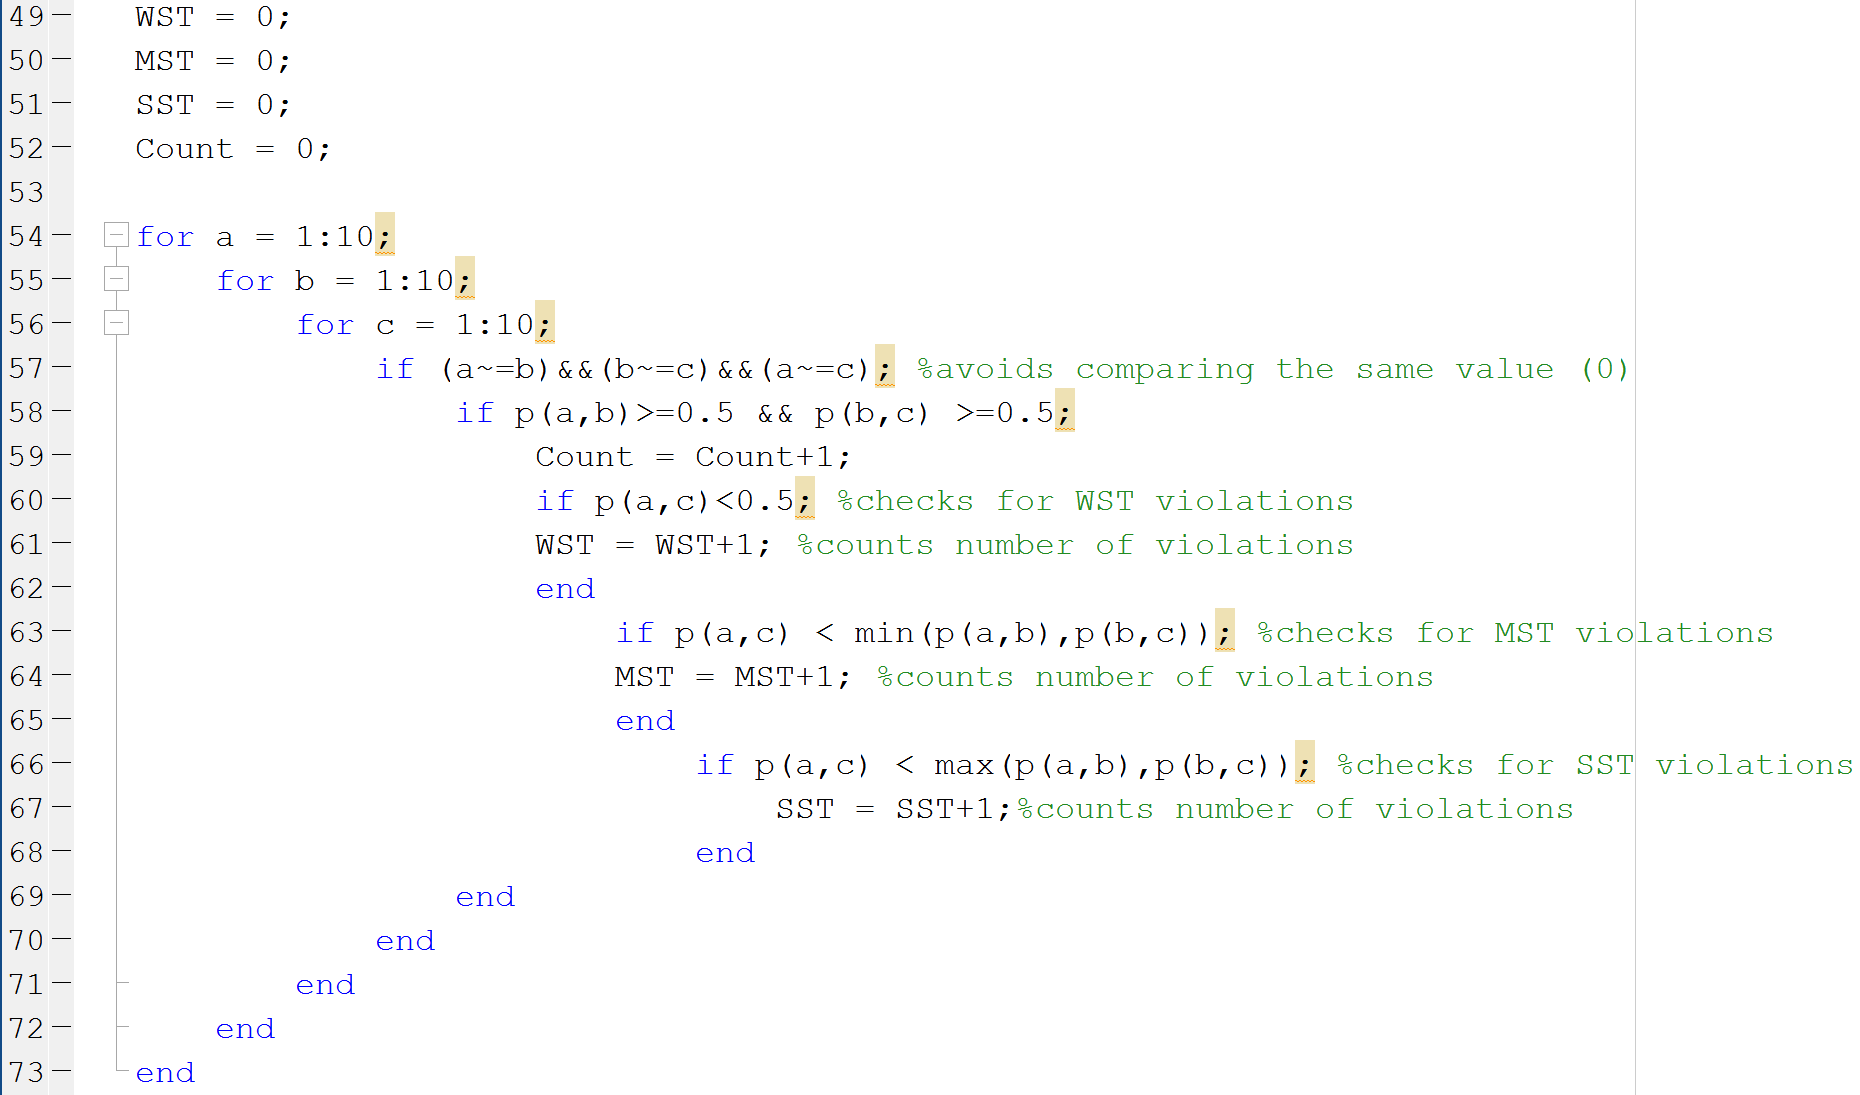
\includegraphics[width = \textwidth]{Figure/loop.png} 
\caption{Loop used to calculate WST, MST and SST violations.}
\label{fig:loop}
\end{figure}
\noindent
%
The same goes for the likelihood estimation. The \textit{fOptiPt.m} Matlab function has been developed for this purpose. The function requires two mandatory input, \textit{M} and \textit{A}, where \textit{M} is the paired comparison matrix shown in \autoref{tab:data}, and \textit{A} is a cell array with length corresponding to the number of stimuli, which is 10. Further there is an optional input, \textit{s}, which denotes the starting values for the estimation routine. The search algorithm starts at $\frac{1}{k}$ for each parameter value, where \textit{k} is the number of parameters, if \textit{s} is not specified. In this case \textit{s} is not specified nor is it used.
\vfill


\section*{Results}
\label{Results}
%

\section*{Discussion}
\label{discussion}
%
%SAftig er der svaret det samme til = den er lige meget. 
From the three dimensional bi-plot it looks like the attributes “Nærende”, “Mættende”, and “Skorpe” are highly correlated, therefore one of these three attributes might be redundant. 
When attributes are highly correlated it can in some cases mean that they measure the same thing. To determine whether or not the three attributes are measuring the same thing, each one of them will be discussed. \blankline
%
The first attribute to be discussed will be "Skorpe''. This is from the category Direct Perception and describes a very superficial element of the buns. It is very unlikely that this attribute is measuring the same thing as the other two, because there is a possibility that a bun can look like something on the outside and then when you see the inside it looks totally different. \blankline
%
The other two attributes are “Nærende” and “Mættende”. The two words are not the same, but it is relevant to take into account that the test subjects of this study did not taste the buns, but only looked and felt the buns. Because the subjects did not taste the buns it could be argued that the attributes “Nærende” and “Mættende” are almost the same. They are both from the category Reflection and they are both related to what you get out of eating the bun. \blankline
%
The attribute "Saftig" does not really contribute to any of the three principal components and the rating of this attribute doesn't vary that much between the different buns either. The reason for the lack of variation for the rating on this attribute is not determined. There is a possibility that it is just because the buns are equally juicy. So if a totally different bun were presented, it could possible vary from the buns used in this study. It could also mean that the participants did not know how to rate a bun on an attribute as "Saftig" when only exposed to a picture.



% An example of a floating figure using the graphicx package.
% Note that \label must occur AFTER (or within) \caption.
% For figures, \caption should occur after the \includegraphics.
% Note that IEEEtran v1.7 and later has special internal code that
% is designed to preserve the operation of \label within \caption
% even when the captionsoff option is in effect. However, because
% of issues like this, it may be the safest practice to put all your
% \label just after \caption rather than within \caption{}.
%
% Reminder: the "draftcls" or "draftclsnofoot", not "draft", class
% option should be used if it is desired that the figures are to be
% displayed while in draft mode.
%
%\begin{figure}[!t]
%\centering
%\includegraphics[width=2.5in]{myfigure}
% where an .eps filename suffix will be assumed under latex, 
% and a .pdf suffix will be assumed for pdflatex; or what has been declared
% via \DeclareGraphicsExtensions.
%\caption{Simulation results for the network.}
%\label{fig_sim}
%\end{figure}

% Note that the IEEE typically puts floats only at the top, even when this
% results in a large percentage of a column being occupied by floats.


% An example of a double column floating figure using two subfigures.
% (The subfig.sty package must be loaded for this to work.)
% The subfigure \label commands are set within each subfloat command,
% and the \label for the overall figure must come after \caption.
% \hfil is used as a separator to get equal spacing.
% Watch out that the combined width of all the subfigures on a 
% line do not exceed the text width or a line break will occur.
%
%\begin{figure*}[!t]
%\centering
%\subfloat[Case I]{\includegraphics[width=2.5in]{box}%
%\label{fig_first_case}}
%\hfil
%\subfloat[Case II]{\includegraphics[width=2.5in]{box}%
%\label{fig_second_case}}
%\caption{Simulation results for the network.}
%\label{fig_sim}
%\end{figure*}
%
% Note that often IEEE papers with subfigures do not employ subfigure
% captions (using the optional argument to \subfloat[]), but instead will
% reference/describe all of them (a), (b), etc., within the main caption.
% Be aware that for subfig.sty to generate the (a), (b), etc., subfigure
% labels, the optional argument to \subfloat must be present. If a
% subcaption is not desired, just leave its contents blank,
% e.g., \subfloat[].


% An example of a floating table. Note that, for IEEE style tables, the
% \caption command should come BEFORE the table and, given that table
% captions serve much like titles, are usually capitalized except for words
% such as a, an, and, as, at, but, by, for, in, nor, of, on, or, the, to
% and up, which are usually not capitalized unless they are the first or
% last word of the caption. Table text will default to \footnotesize as
% the IEEE normally uses this smaller font for tables.
% The \label must come after \caption as always.
%
%\begin{table}[!t]
%% increase table row spacing, adjust to taste
%\renewcommand{\arraystretch}{1.3}
% if using array.sty, it might be a good idea to tweak the value of
% \extrarowheight as needed to properly center the text within the cells
%\caption{An Example of a Table}
%\label{table_example}
%\centering
%% Some packages, such as MDW tools, offer better commands for making tables
%% than the plain LaTeX2e tabular which is used here.
%\begin{tabular}{|c||c|}
%\hline
%One & Two\\
%\hline
%Three & Four\\
%\hline
%\end{tabular}
%\end{table}


% Note that the IEEE does not put floats in the very first column
% - or typically anywhere on the first page for that matter. Also,
% in-text middle ("here") positioning is typically not used, but it
% is allowed and encouraged for Computer Society conferences (but
% not Computer Society journals). Most IEEE journals/conferences use
% top floats exclusively. 
% Note that, LaTeX2e, unlike IEEE journals/conferences, places
% footnotes above bottom floats. This can be corrected via the
% \fnbelowfloat command of the stfloats package.



\section*{Conclusion}
%





% conference papers do not normally have an appendix


% use section* for acknowledgment
% use section* for acknowledgment
\section*{Acknowledgment}
\label{Acknowledgment}
%
The authors would like to thank...


The authors would like to thank...  \cite{Graaf2013} og \cite{Graaf2015}






% trigger a \newpage just before the given reference
% number - used to balance the columns on the last page
% adjust value as needed - may need to be readjusted if
% the document is modified later
%\IEEEtriggeratref{8}
% The "triggered" command can be changed if desired:
%\IEEEtriggercmd{\enlargethispage{-5in}}

% references section

% can use a bibliography generated by BibTeX as a .bbl file
% BibTeX documentation can be easily obtained at:
% http://mirror.ctan.org/biblio/bibtex/contrib/doc/
% The IEEEtran BibTeX style support page is at:
% http://www.michaelshell.org/tex/ieeetran/bibtex/
\bibliographystyle{IEEEtran}
% argument is your BibTeX string definitions and bibliography database(s)
\bibliography{References}
%
% <OR> manually copy in the resultant .bbl file
% set second argument of \begin to the number of references
% (used to reserve space for the reference number labels box)
%\begin{thebibliography}{1}
%
%\bibitem{IEEEhowto:kopka}
%H.~Kopka and P.~W. Daly, \emph{A Guide to \LaTeX}, 3rd~ed.\hskip 1em plus
%  0.5em minus 0.4em\relax Harlow, England: Addison-Wesley, 1999.
%\end{thebibliography}




% that's all folks
\end{document}


